\documentclass{article}\usepackage[]{graphicx}\usepackage[]{color}
%% maxwidth is the original width if it is less than linewidth
%% otherwise use linewidth (to make sure the graphics do not exceed the margin)
\makeatletter
\def\maxwidth{ %
  \ifdim\Gin@nat@width>\linewidth
    \linewidth
  \else
    \Gin@nat@width
  \fi
}
\makeatother

\definecolor{fgcolor}{rgb}{0.345, 0.345, 0.345}
\newcommand{\hlnum}[1]{\textcolor[rgb]{0.686,0.059,0.569}{#1}}%
\newcommand{\hlstr}[1]{\textcolor[rgb]{0.192,0.494,0.8}{#1}}%
\newcommand{\hlcom}[1]{\textcolor[rgb]{0.678,0.584,0.686}{\textit{#1}}}%
\newcommand{\hlopt}[1]{\textcolor[rgb]{0,0,0}{#1}}%
\newcommand{\hlstd}[1]{\textcolor[rgb]{0.345,0.345,0.345}{#1}}%
\newcommand{\hlkwa}[1]{\textcolor[rgb]{0.161,0.373,0.58}{\textbf{#1}}}%
\newcommand{\hlkwb}[1]{\textcolor[rgb]{0.69,0.353,0.396}{#1}}%
\newcommand{\hlkwc}[1]{\textcolor[rgb]{0.333,0.667,0.333}{#1}}%
\newcommand{\hlkwd}[1]{\textcolor[rgb]{0.737,0.353,0.396}{\textbf{#1}}}%

\usepackage{framed}
\makeatletter
\newenvironment{kframe}{%
 \def\at@end@of@kframe{}%
 \ifinner\ifhmode%
  \def\at@end@of@kframe{\end{minipage}}%
  \begin{minipage}{\columnwidth}%
 \fi\fi%
 \def\FrameCommand##1{\hskip\@totalleftmargin \hskip-\fboxsep
 \colorbox{shadecolor}{##1}\hskip-\fboxsep
     % There is no \\@totalrightmargin, so:
     \hskip-\linewidth \hskip-\@totalleftmargin \hskip\columnwidth}%
 \MakeFramed {\advance\hsize-\width
   \@totalleftmargin\z@ \linewidth\hsize
   \@setminipage}}%
 {\par\unskip\endMakeFramed%
 \at@end@of@kframe}
\makeatother

\definecolor{shadecolor}{rgb}{.97, .97, .97}
\definecolor{messagecolor}{rgb}{0, 0, 0}
\definecolor{warningcolor}{rgb}{1, 0, 1}
\definecolor{errorcolor}{rgb}{1, 0, 0}
\newenvironment{knitrout}{}{} % an empty environment to be redefined in TeX

\usepackage{alltt}
\usepackage[T1]{fontenc}
\usepackage{datetime}
\usepackage[margin=1in]{geometry}

\newcommand{\qu}[1]{``#1''}%

\title{Simulation Result Report}
\author{Adam Kapelner}
\date{\today, \currenttime}
\IfFileExists{upquote.sty}{\usepackage{upquote}}{}
\begin{document}
\maketitle






\section{Results for each Run}

\begin{knitrout}
\definecolor{shadecolor}{rgb}{0.969, 0.969, 0.969}\color{fgcolor}
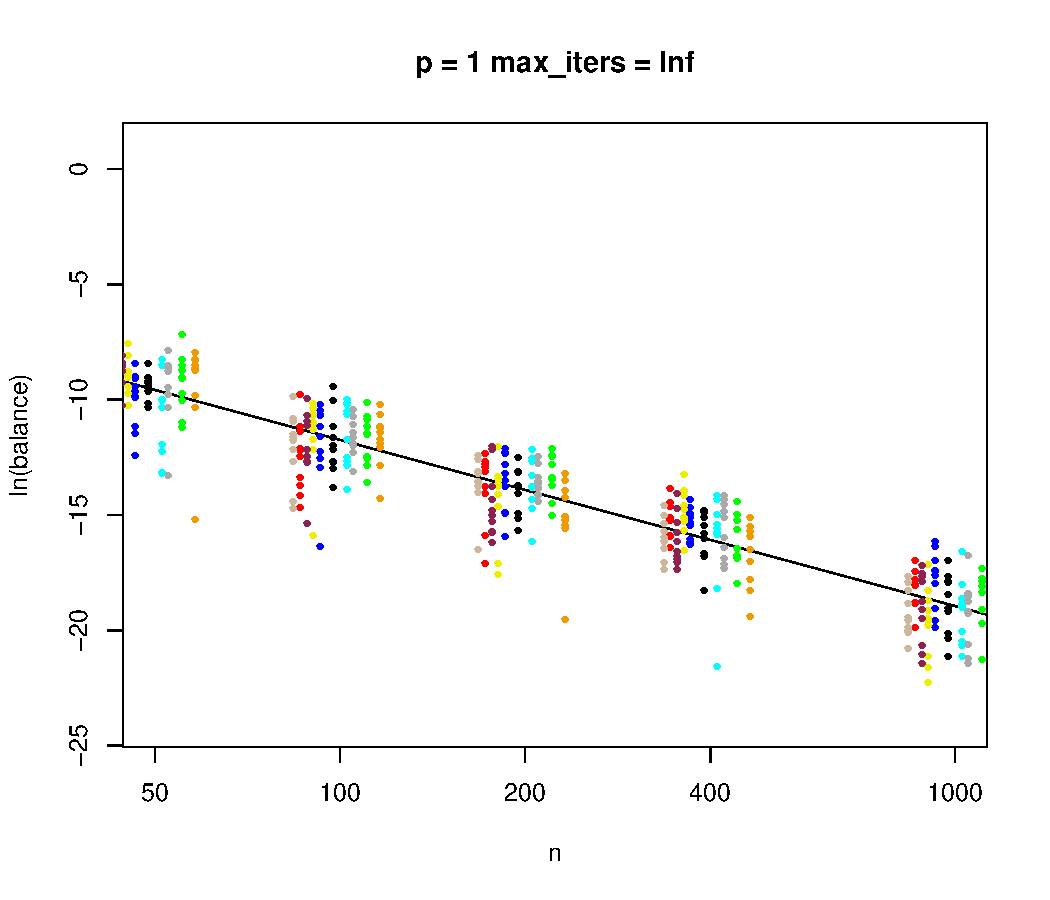
\includegraphics[width=\maxwidth]{figure/load_and_cleanup_data1} 
\begin{kframe}\begin{verbatim}
## p = 1 max iters = Inf 
## 
## 
## examine log-log linear regression
##             Estimate Std. Error t value   Pr(>|t|)
## (Intercept)    2.648    0.32724   8.092  4.538e-15
## lnx           -3.126    0.06011 -52.008 2.093e-203
## ensure log-law relationship
## Analysis of Variance Table
## 
## Model 1: lny ~ poly(lnx, 1)
## Model 2: lny ~ poly(lnx, 4)
##   Res.Df RSS Df Sum of Sq    F Pr(>F)  
## 1    498 983                           
## 2    495 970  3      12.5 2.12  0.096 .
## ---
## Signif. codes:  0 '***' 0.001 '**' 0.01 '*' 0.05 '.' 0.1 ' ' 1
## ensure no dataset effect
## Analysis of Variance Table
## 
## Model 1: lny ~ lnx
## Model 2: lny ~ lnx + dataset
##   Res.Df RSS Df Sum of Sq    F Pr(>F)  
## 1    498 983                           
## 2    489 942  9      40.6 2.34  0.014 *
## ---
## Signif. codes:  0 '***' 0.001 '**' 0.01 '*' 0.05 '.' 0.1 ' ' 1
## Analysis of Variance Table
## 
## Model 1: lny ~ lnx
## Model 2: lny ~ lnx * dataset
##   Res.Df RSS Df Sum of Sq    F  Pr(>F)    
## 1    498 983                              
## 2    480 879 18       104 3.17 1.4e-05 ***
## ---
## Signif. codes:  0 '***' 0.001 '**' 0.01 '*' 0.05 '.' 0.1 ' ' 1
\end{verbatim}
\end{kframe}
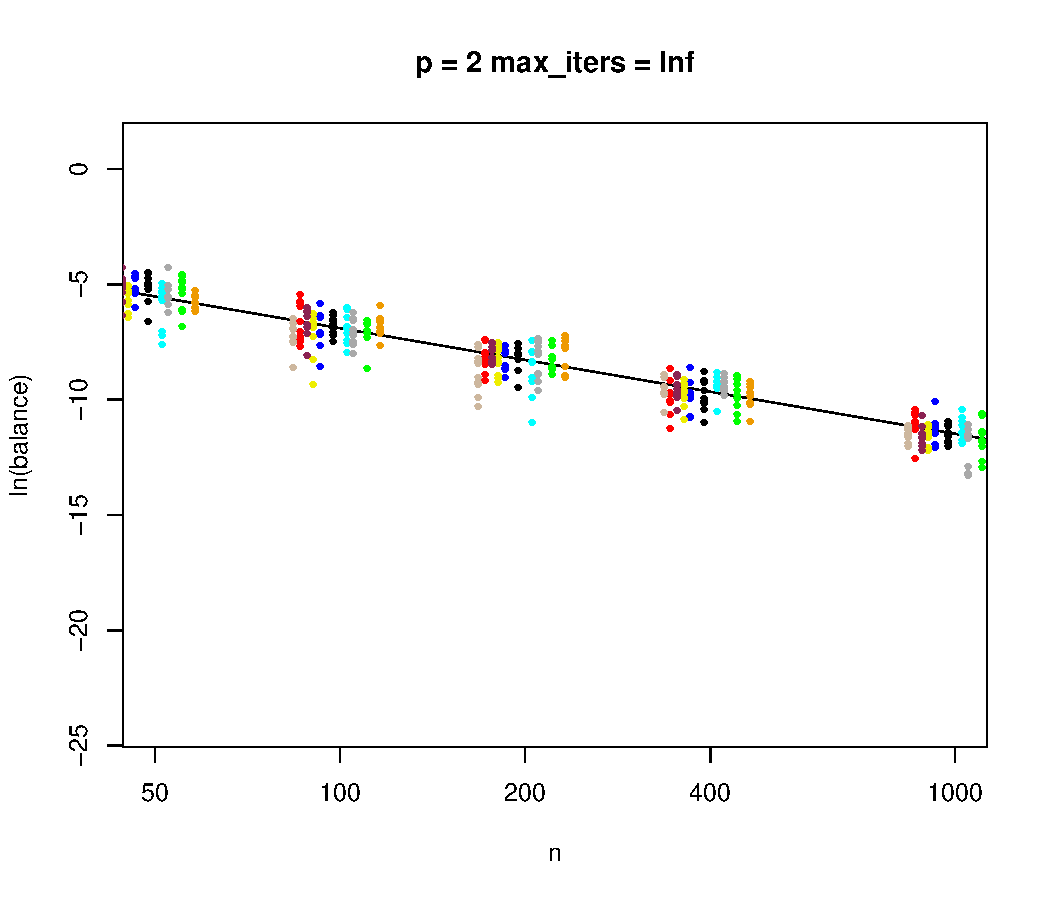
\includegraphics[width=\maxwidth]{figure/load_and_cleanup_data2} 
\begin{kframe}\begin{verbatim}
## p = 2 max iters = Inf 
## 
## 
## examine log-log linear regression
##             Estimate Std. Error t value   Pr(>|t|)
## (Intercept)    2.240     0.1476   15.18  4.707e-43
## lnx           -1.986     0.0271  -73.27 6.995e-269
## ensure log-law relationship
## Analysis of Variance Table
## 
## Model 1: lny ~ poly(lnx, 1)
## Model 2: lny ~ poly(lnx, 4)
##   Res.Df RSS Df Sum of Sq    F Pr(>F)
## 1    498 200                         
## 2    495 199  3     0.553 0.46   0.71
## ensure no dataset effect
## Analysis of Variance Table
## 
## Model 1: lny ~ lnx
## Model 2: lny ~ lnx + dataset
##   Res.Df RSS Df Sum of Sq    F Pr(>F)
## 1    498 200                         
## 2    489 195  9      4.56 1.27   0.25
## Analysis of Variance Table
## 
## Model 1: lny ~ lnx
## Model 2: lny ~ lnx * dataset
##   Res.Df RSS Df Sum of Sq    F Pr(>F)  
## 1    498 200                           
## 2    480 188 18      12.2 1.73  0.031 *
## ---
## Signif. codes:  0 '***' 0.001 '**' 0.01 '*' 0.05 '.' 0.1 ' ' 1
\end{verbatim}
\end{kframe}
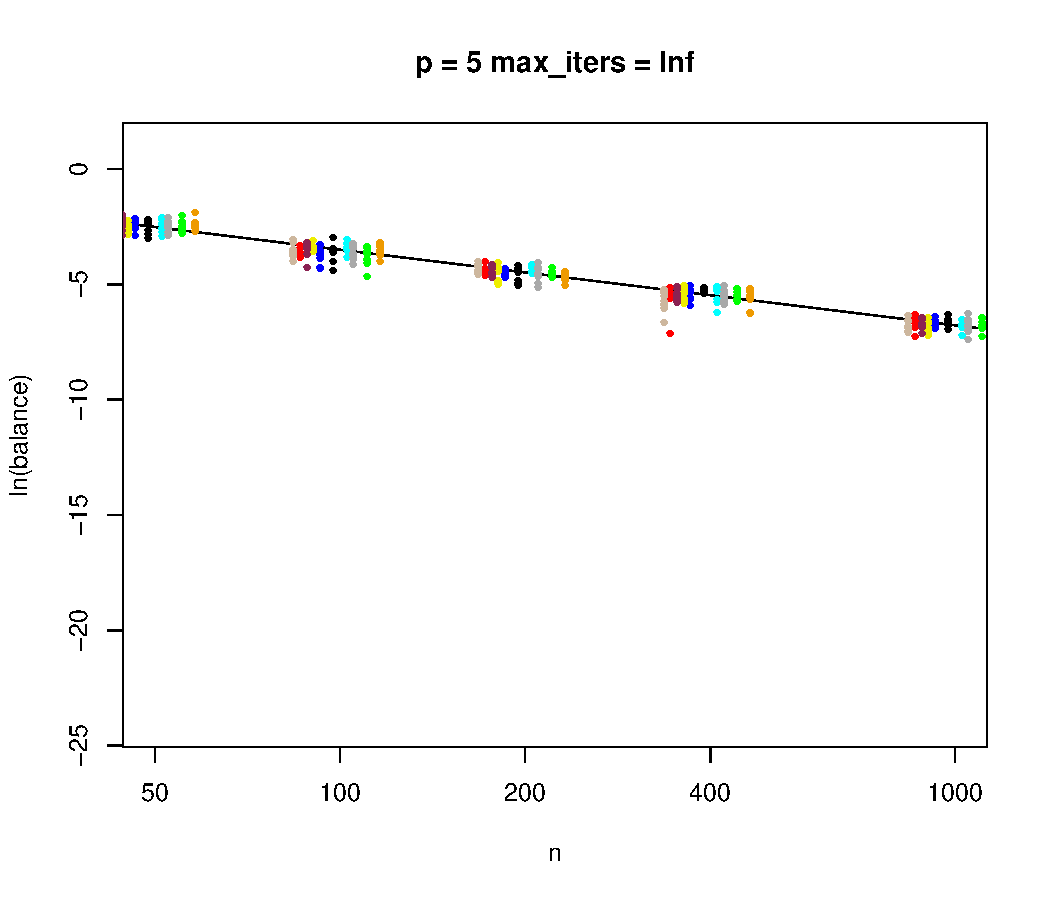
\includegraphics[width=\maxwidth]{figure/load_and_cleanup_data3} 
\begin{kframe}\begin{verbatim}
## p = 5 max iters = Inf 
## 
## 
## examine log-log linear regression
##             Estimate Std. Error t value   Pr(>|t|)
## (Intercept)    3.041    0.06357   47.84 2.432e-188
## lnx           -1.421    0.01168 -121.74  0.000e+00
## ensure log-law relationship
## Analysis of Variance Table
## 
## Model 1: lny ~ poly(lnx, 1)
## Model 2: lny ~ poly(lnx, 4)
##   Res.Df  RSS Df Sum of Sq    F  Pr(>F)    
## 1    498 37.1                              
## 2    495 35.8  3      1.32 6.07 0.00046 ***
## ---
## Signif. codes:  0 '***' 0.001 '**' 0.01 '*' 0.05 '.' 0.1 ' ' 1
## ensure no dataset effect
## Analysis of Variance Table
## 
## Model 1: lny ~ lnx
## Model 2: lny ~ lnx + dataset
##   Res.Df  RSS Df Sum of Sq    F Pr(>F)
## 1    498 37.1                         
## 2    489 36.2  9     0.853 1.28   0.25
## Analysis of Variance Table
## 
## Model 1: lny ~ lnx
## Model 2: lny ~ lnx * dataset
##   Res.Df  RSS Df Sum of Sq    F Pr(>F)
## 1    498 37.1                         
## 2    480 35.6 18      1.46 1.09   0.36
\end{verbatim}
\end{kframe}
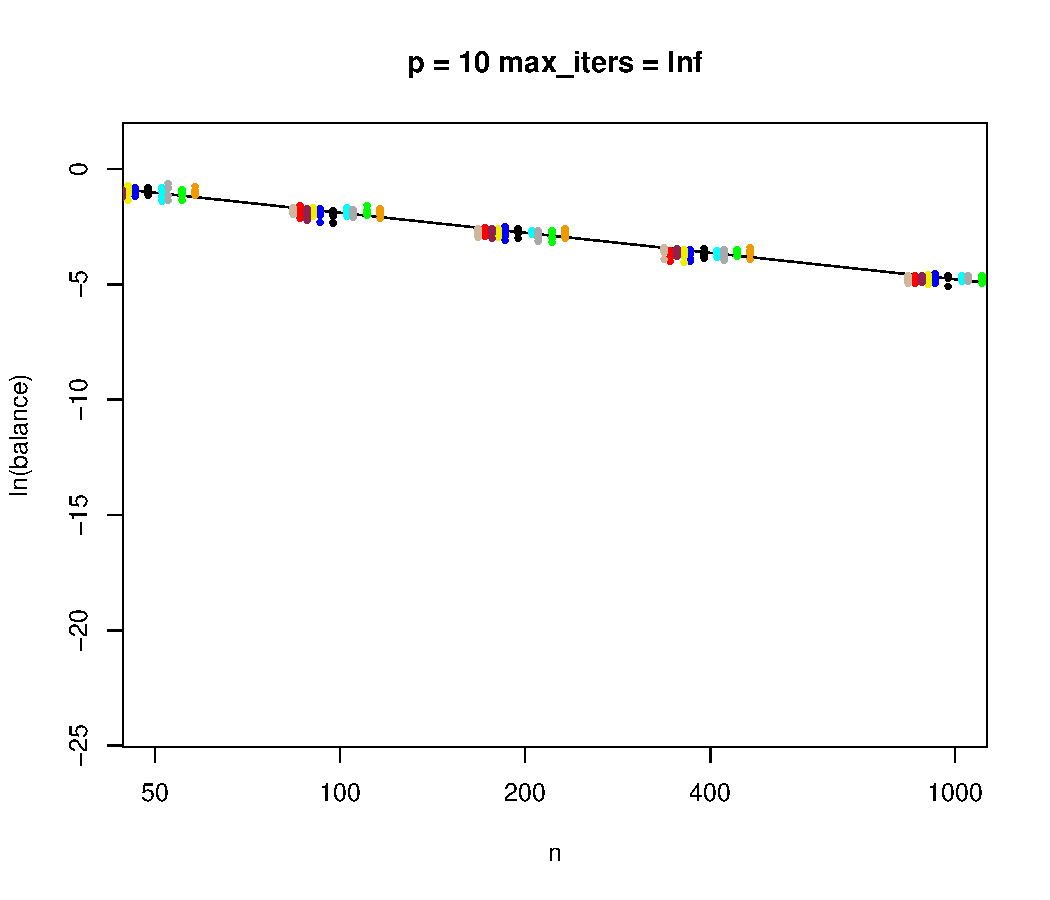
\includegraphics[width=\maxwidth]{figure/load_and_cleanup_data4} 
\begin{kframe}\begin{verbatim}
## p = 10 max iters = Inf 
## 
## 
## examine log-log linear regression
##             Estimate Std. Error t value Pr(>|t|)
## (Intercept)    3.864   0.032841   117.7        0
## lnx           -1.252   0.006032  -207.6        0
## ensure log-law relationship
## Analysis of Variance Table
## 
## Model 1: lny ~ poly(lnx, 1)
## Model 2: lny ~ poly(lnx, 4)
##   Res.Df  RSS Df Sum of Sq    F Pr(>F)
## 1    498 9.90                         
## 2    495 9.81  3    0.0948 1.59   0.19
## ensure no dataset effect
## Analysis of Variance Table
## 
## Model 1: lny ~ lnx
## Model 2: lny ~ lnx + dataset
##   Res.Df  RSS Df Sum of Sq    F Pr(>F)
## 1    498 9.90                         
## 2    489 9.68  9     0.224 1.26   0.26
## Analysis of Variance Table
## 
## Model 1: lny ~ lnx
## Model 2: lny ~ lnx * dataset
##   Res.Df  RSS Df Sum of Sq    F Pr(>F)
## 1    498 9.90                         
## 2    480 9.53 18     0.367 1.03   0.43
\end{verbatim}
\end{kframe}
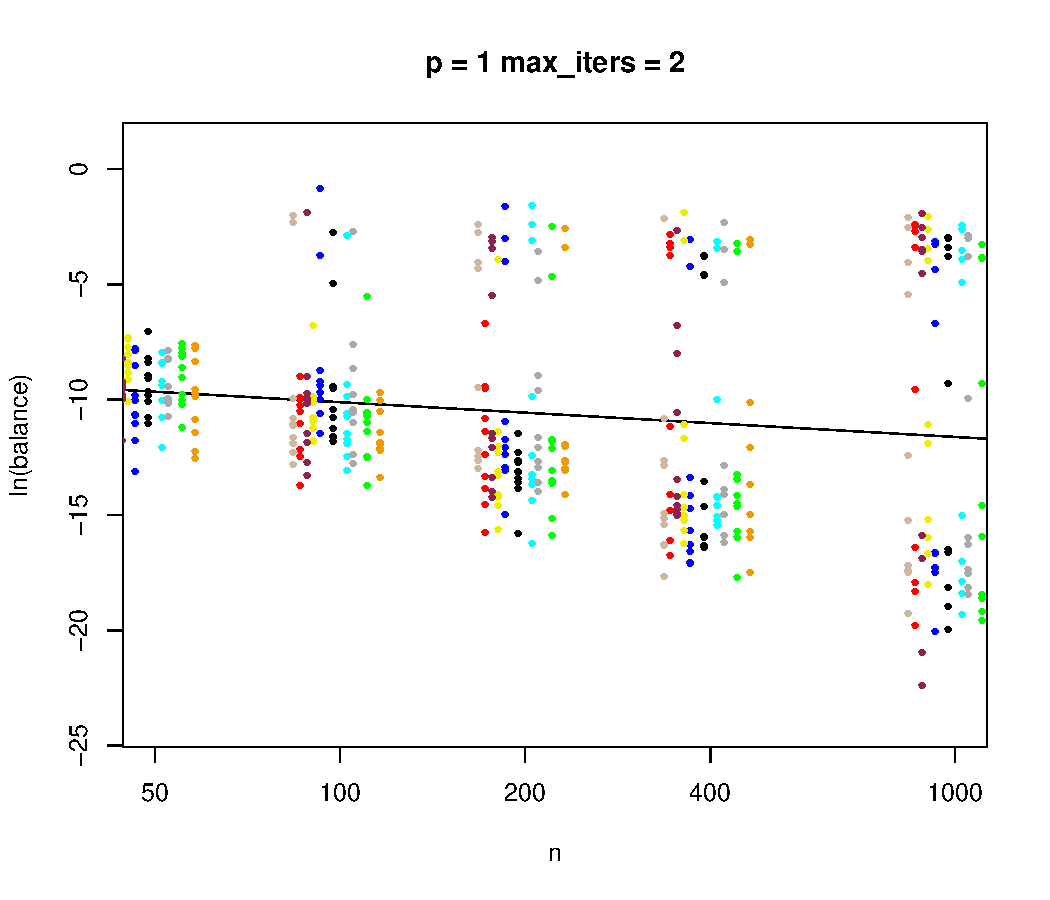
\includegraphics[width=\maxwidth]{figure/load_and_cleanup_data5} 
\begin{kframe}\begin{verbatim}
## p = 1 max iters = 2 
## 
## 
## examine log-log linear regression
##             Estimate Std. Error t value  Pr(>|t|)
## (Intercept)   -7.102     1.0602  -6.699 5.691e-11
## lnx           -0.654     0.1947  -3.358 8.441e-04
## ensure log-law relationship
## Analysis of Variance Table
## 
## Model 1: lny ~ poly(lnx, 1)
## Model 2: lny ~ poly(lnx, 4)
##   Res.Df   RSS Df Sum of Sq    F Pr(>F)  
## 1    498 10316                           
## 2    495 10163  3       153 2.48   0.06 .
## ---
## Signif. codes:  0 '***' 0.001 '**' 0.01 '*' 0.05 '.' 0.1 ' ' 1
## ensure no dataset effect
## Analysis of Variance Table
## 
## Model 1: lny ~ lnx
## Model 2: lny ~ lnx + dataset
##   Res.Df   RSS Df Sum of Sq   F Pr(>F)
## 1    498 10316                        
## 2    489 10260  9      56.6 0.3   0.97
## Analysis of Variance Table
## 
## Model 1: lny ~ lnx
## Model 2: lny ~ lnx * dataset
##   Res.Df   RSS Df Sum of Sq    F Pr(>F)
## 1    498 10316                         
## 2    480 10135 18       182 0.48   0.97
\end{verbatim}
\end{kframe}
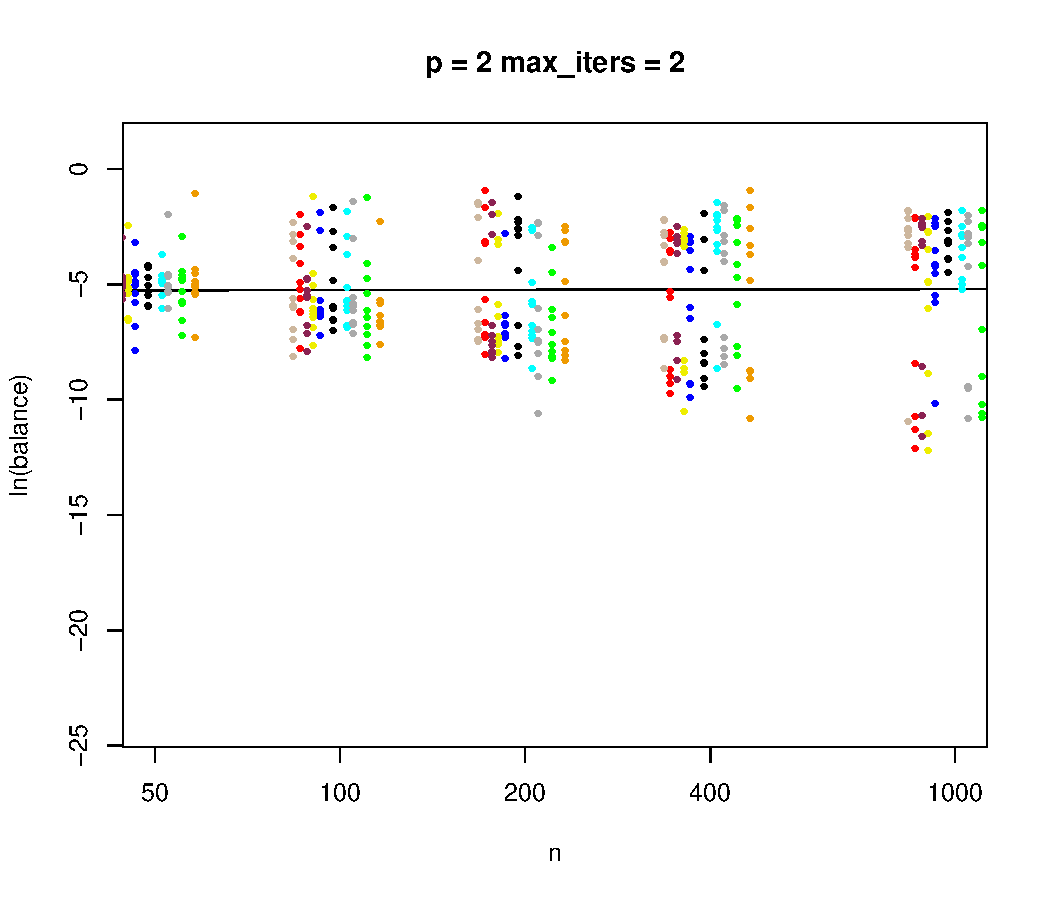
\includegraphics[width=\maxwidth]{figure/load_and_cleanup_data6} 
\begin{kframe}\begin{verbatim}
## p = 2 max iters = 2 
## 
## 
## examine log-log linear regression
##             Estimate Std. Error t value  Pr(>|t|)
## (Intercept) -5.33102     0.5592 -9.5338 6.686e-20
## lnx          0.01698     0.1027  0.1653 8.687e-01
## ensure log-law relationship
## Analysis of Variance Table
## 
## Model 1: lny ~ poly(lnx, 1)
## Model 2: lny ~ poly(lnx, 4)
##   Res.Df  RSS Df Sum of Sq    F Pr(>F)  
## 1    498 2870                           
## 2    495 2831  3      39.1 2.28  0.079 .
## ---
## Signif. codes:  0 '***' 0.001 '**' 0.01 '*' 0.05 '.' 0.1 ' ' 1
## ensure no dataset effect
## Analysis of Variance Table
## 
## Model 1: lny ~ lnx
## Model 2: lny ~ lnx + dataset
##   Res.Df  RSS Df Sum of Sq   F Pr(>F)  
## 1    498 2870                          
## 2    489 2783  9      87.3 1.7  0.085 .
## ---
## Signif. codes:  0 '***' 0.001 '**' 0.01 '*' 0.05 '.' 0.1 ' ' 1
## Analysis of Variance Table
## 
## Model 1: lny ~ lnx
## Model 2: lny ~ lnx * dataset
##   Res.Df  RSS Df Sum of Sq    F Pr(>F)  
## 1    498 2870                           
## 2    480 2697 18       173 1.71  0.034 *
## ---
## Signif. codes:  0 '***' 0.001 '**' 0.01 '*' 0.05 '.' 0.1 ' ' 1
\end{verbatim}
\end{kframe}
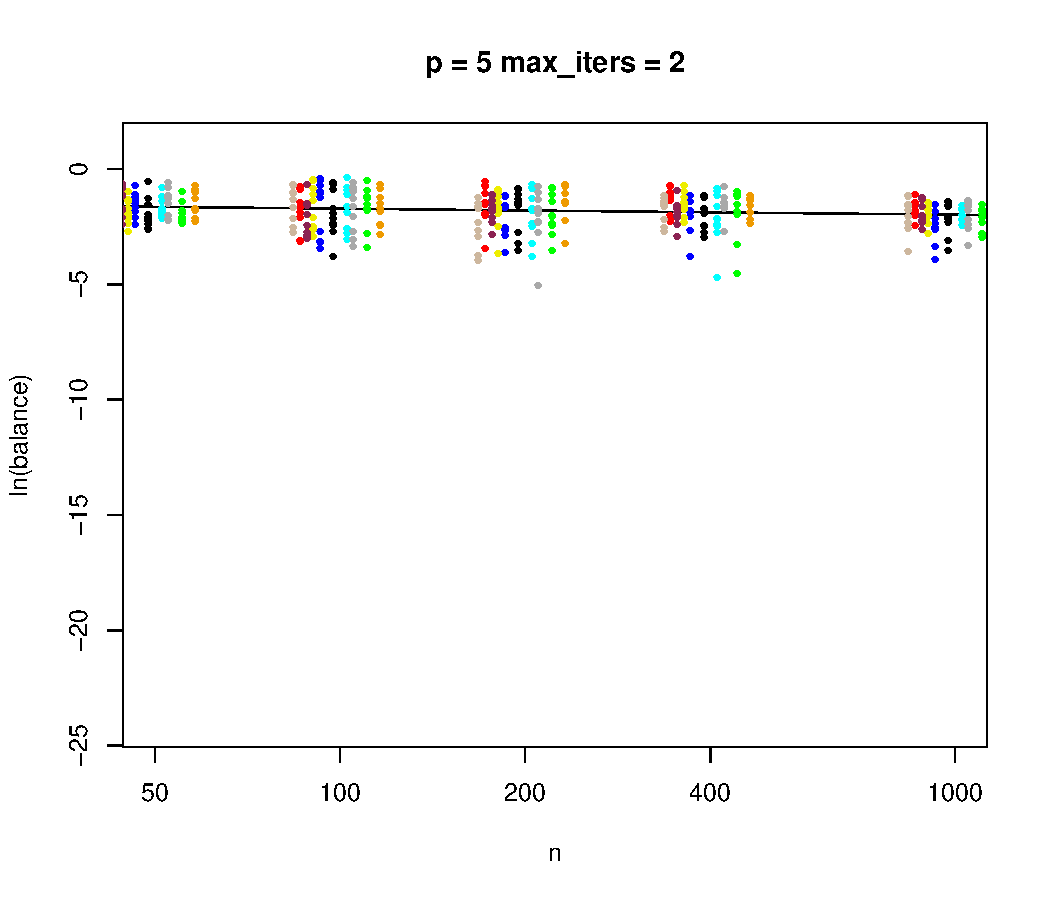
\includegraphics[width=\maxwidth]{figure/load_and_cleanup_data7} 
\begin{kframe}\begin{verbatim}
## p = 5 max iters = 2 
## 
## 
## examine log-log linear regression
##             Estimate Std. Error t value  Pr(>|t|)
## (Intercept)  -1.1958    0.17517  -6.827 2.537e-11
## lnx          -0.1145    0.03218  -3.560 4.065e-04
## ensure log-law relationship
## Analysis of Variance Table
## 
## Model 1: lny ~ poly(lnx, 1)
## Model 2: lny ~ poly(lnx, 4)
##   Res.Df RSS Df Sum of Sq    F Pr(>F)
## 1    498 282                         
## 2    495 280  3      1.59 0.94   0.42
## ensure no dataset effect
## Analysis of Variance Table
## 
## Model 1: lny ~ lnx
## Model 2: lny ~ lnx + dataset
##   Res.Df RSS Df Sum of Sq    F Pr(>F)
## 1    498 282                         
## 2    489 273  9      8.21 1.63    0.1
## Analysis of Variance Table
## 
## Model 1: lny ~ lnx
## Model 2: lny ~ lnx * dataset
##   Res.Df RSS Df Sum of Sq    F Pr(>F)
## 1    498 282                         
## 2    480 270 18      11.9 1.18   0.27
\end{verbatim}
\end{kframe}
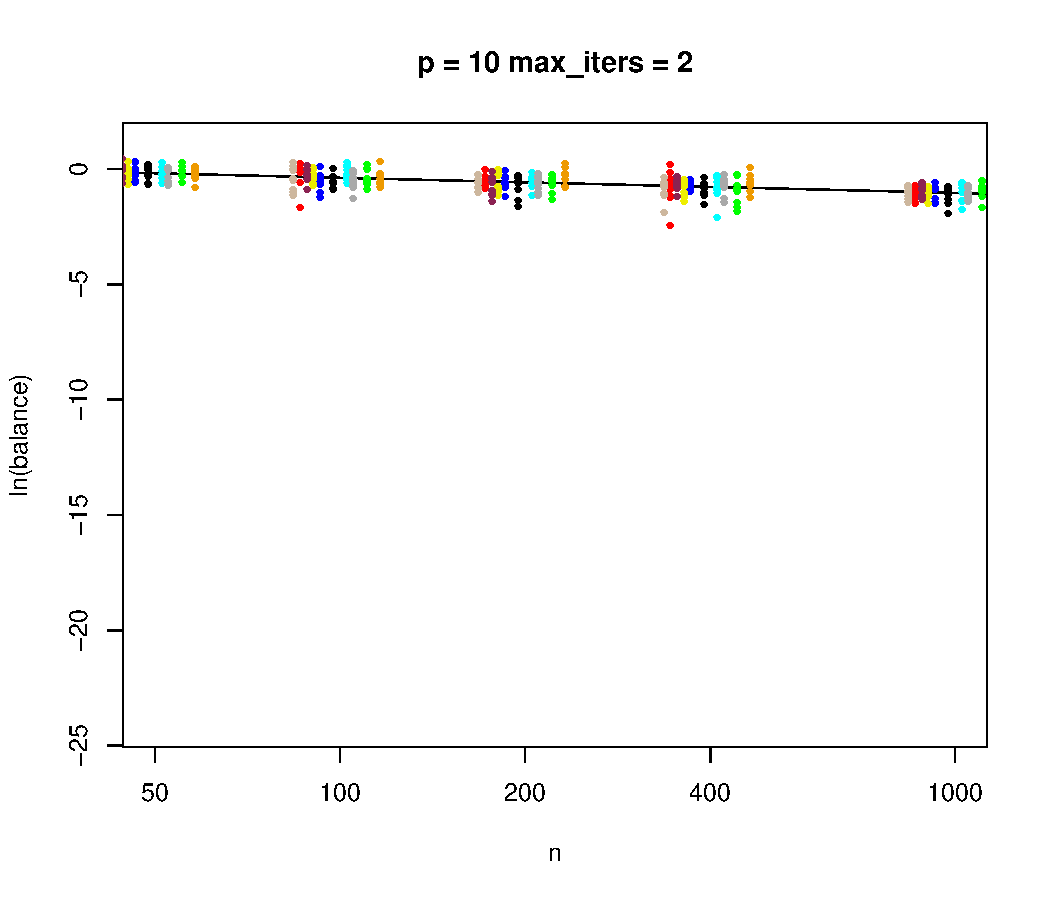
\includegraphics[width=\maxwidth]{figure/load_and_cleanup_data8} 
\begin{kframe}\begin{verbatim}
## p = 10 max iters = 2 
## 
## 
## examine log-log linear regression
##             Estimate Std. Error t value  Pr(>|t|)
## (Intercept)   0.9213    0.08125   11.34 1.141e-26
## lnx          -0.2839    0.01492  -19.02 4.686e-61
## ensure log-law relationship
## Analysis of Variance Table
## 
## Model 1: lny ~ poly(lnx, 1)
## Model 2: lny ~ poly(lnx, 4)
##   Res.Df  RSS Df Sum of Sq    F Pr(>F)
## 1    498 60.6                         
## 2    495 60.5  3     0.123 0.34    0.8
## ensure no dataset effect
## Analysis of Variance Table
## 
## Model 1: lny ~ lnx
## Model 2: lny ~ lnx + dataset
##   Res.Df  RSS Df Sum of Sq    F Pr(>F)
## 1    498 60.6                         
## 2    489 59.3  9      1.24 1.14   0.33
## Analysis of Variance Table
## 
## Model 1: lny ~ lnx
## Model 2: lny ~ lnx * dataset
##   Res.Df  RSS Df Sum of Sq    F Pr(>F)
## 1    498 60.6                         
## 2    480 58.6 18      2.02 0.92   0.55
\end{verbatim}
\end{kframe}
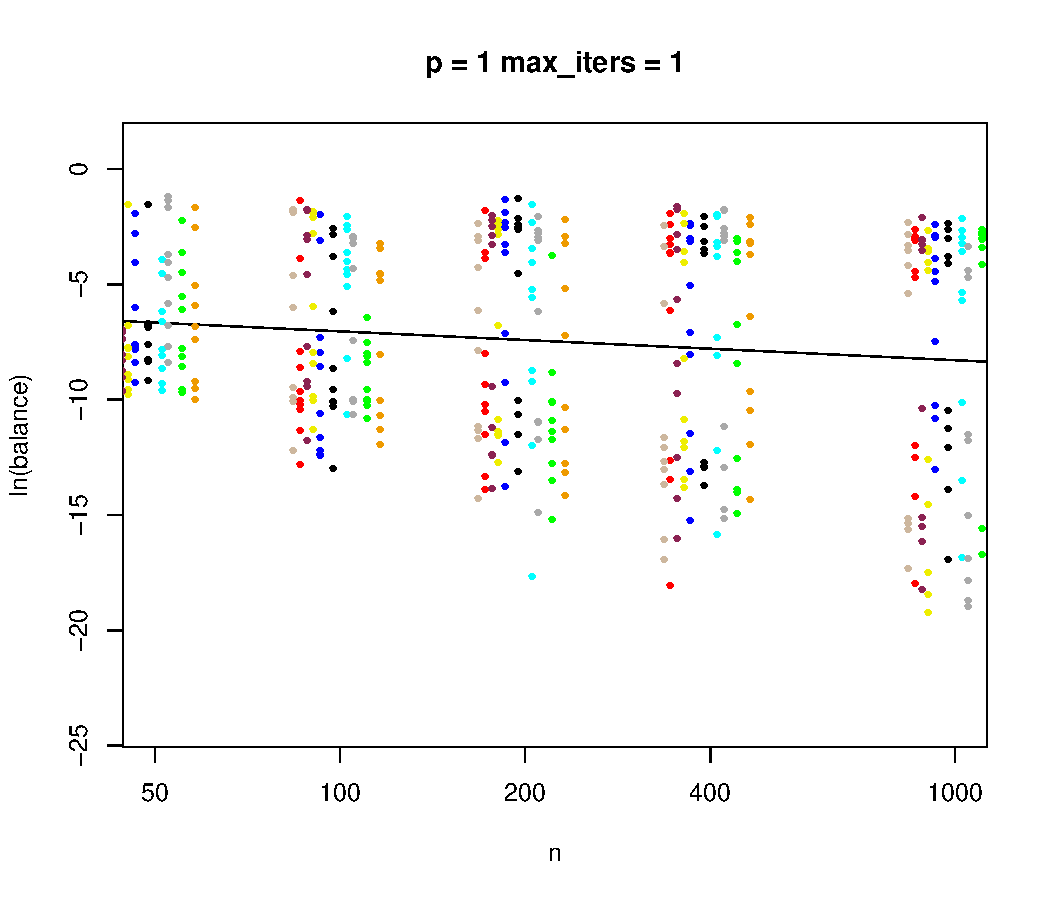
\includegraphics[width=\maxwidth]{figure/load_and_cleanup_data9} 
\begin{kframe}\begin{verbatim}
## p = 1 max iters = 1 
## 
## 
## examine log-log linear regression
##             Estimate Std. Error t value  Pr(>|t|)
## (Intercept)   -4.542      1.045  -4.345 1.692e-05
## lnx           -0.543      0.192  -2.828 4.879e-03
## ensure log-law relationship
## Analysis of Variance Table
## 
## Model 1: lny ~ poly(lnx, 1)
## Model 2: lny ~ poly(lnx, 4)
##   Res.Df   RSS Df Sum of Sq    F Pr(>F)
## 1    498 10032                         
## 2    495 10028  3      4.01 0.07   0.98
## ensure no dataset effect
## Analysis of Variance Table
## 
## Model 1: lny ~ lnx
## Model 2: lny ~ lnx + dataset
##   Res.Df   RSS Df Sum of Sq    F Pr(>F)
## 1    498 10032                         
## 2    489  9914  9       118 0.65   0.76
## Analysis of Variance Table
## 
## Model 1: lny ~ lnx
## Model 2: lny ~ lnx * dataset
##   Res.Df   RSS Df Sum of Sq    F Pr(>F)
## 1    498 10032                         
## 2    480  9616 18       416 1.15    0.3
\end{verbatim}
\end{kframe}
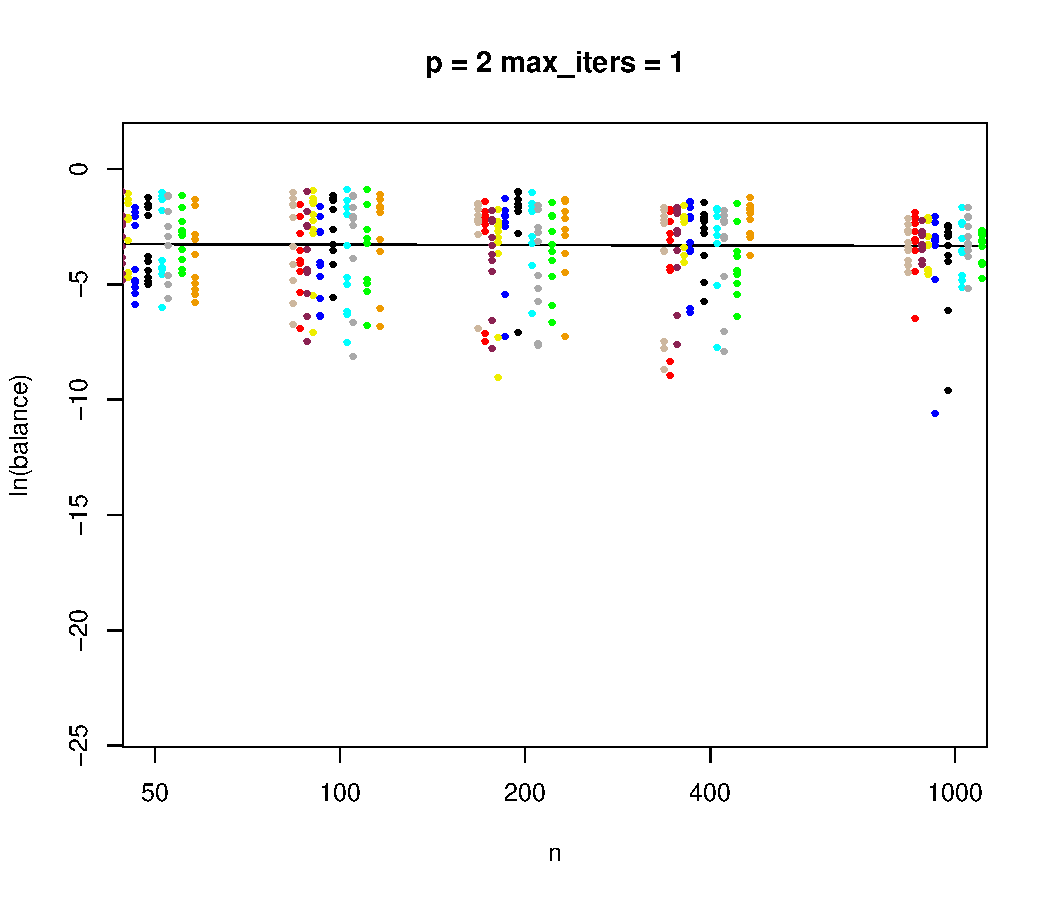
\includegraphics[width=\maxwidth]{figure/load_and_cleanup_data10} 
\begin{kframe}\begin{verbatim}
## p = 2 max iters = 1 
## 
## 
## examine log-log linear regression
##             Estimate Std. Error t value  Pr(>|t|)
## (Intercept) -3.16015    0.40802 -7.7452 5.383e-14
## lnx         -0.02654    0.07494 -0.3541 7.234e-01
## ensure log-law relationship
## Analysis of Variance Table
## 
## Model 1: lny ~ poly(lnx, 1)
## Model 2: lny ~ poly(lnx, 4)
##   Res.Df  RSS Df Sum of Sq    F Pr(>F)
## 1    498 1528                         
## 2    495 1525  3      3.05 0.33    0.8
## ensure no dataset effect
## Analysis of Variance Table
## 
## Model 1: lny ~ lnx
## Model 2: lny ~ lnx + dataset
##   Res.Df  RSS Df Sum of Sq    F Pr(>F)
## 1    498 1528                         
## 2    489 1506  9      21.6 0.78   0.64
## Analysis of Variance Table
## 
## Model 1: lny ~ lnx
## Model 2: lny ~ lnx * dataset
##   Res.Df  RSS Df Sum of Sq   F Pr(>F)
## 1    498 1528                        
## 2    480 1489 18      39.3 0.7   0.81
\end{verbatim}
\end{kframe}
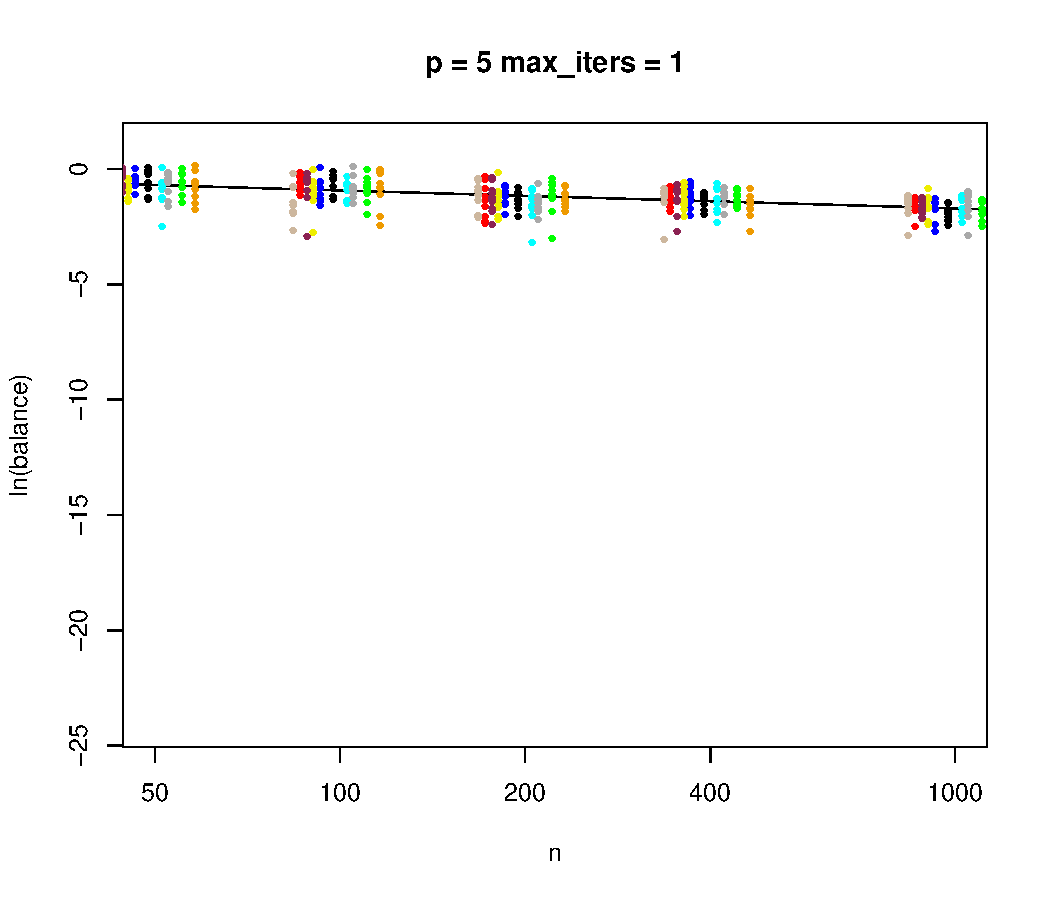
\includegraphics[width=\maxwidth]{figure/load_and_cleanup_data11} 
\begin{kframe}\begin{verbatim}
## p = 5 max iters = 1 
## 
## 
## examine log-log linear regression
##             Estimate Std. Error t value  Pr(>|t|)
## (Intercept)   0.6113    0.12485   4.896 1.322e-06
## lnx          -0.3361    0.02293 -14.656 1.082e-40
## ensure log-law relationship
## Analysis of Variance Table
## 
## Model 1: lny ~ poly(lnx, 1)
## Model 2: lny ~ poly(lnx, 4)
##   Res.Df RSS Df Sum of Sq    F Pr(>F)  
## 1    498 143                           
## 2    495 140  3      2.75 3.23  0.022 *
## ---
## Signif. codes:  0 '***' 0.001 '**' 0.01 '*' 0.05 '.' 0.1 ' ' 1
## ensure no dataset effect
## Analysis of Variance Table
## 
## Model 1: lny ~ lnx
## Model 2: lny ~ lnx + dataset
##   Res.Df RSS Df Sum of Sq   F Pr(>F)
## 1    498 143                        
## 2    489 141  9      2.33 0.9   0.53
## Analysis of Variance Table
## 
## Model 1: lny ~ lnx
## Model 2: lny ~ lnx * dataset
##   Res.Df RSS Df Sum of Sq    F Pr(>F)
## 1    498 143                         
## 2    480 137 18      6.27 1.22   0.24
\end{verbatim}
\end{kframe}
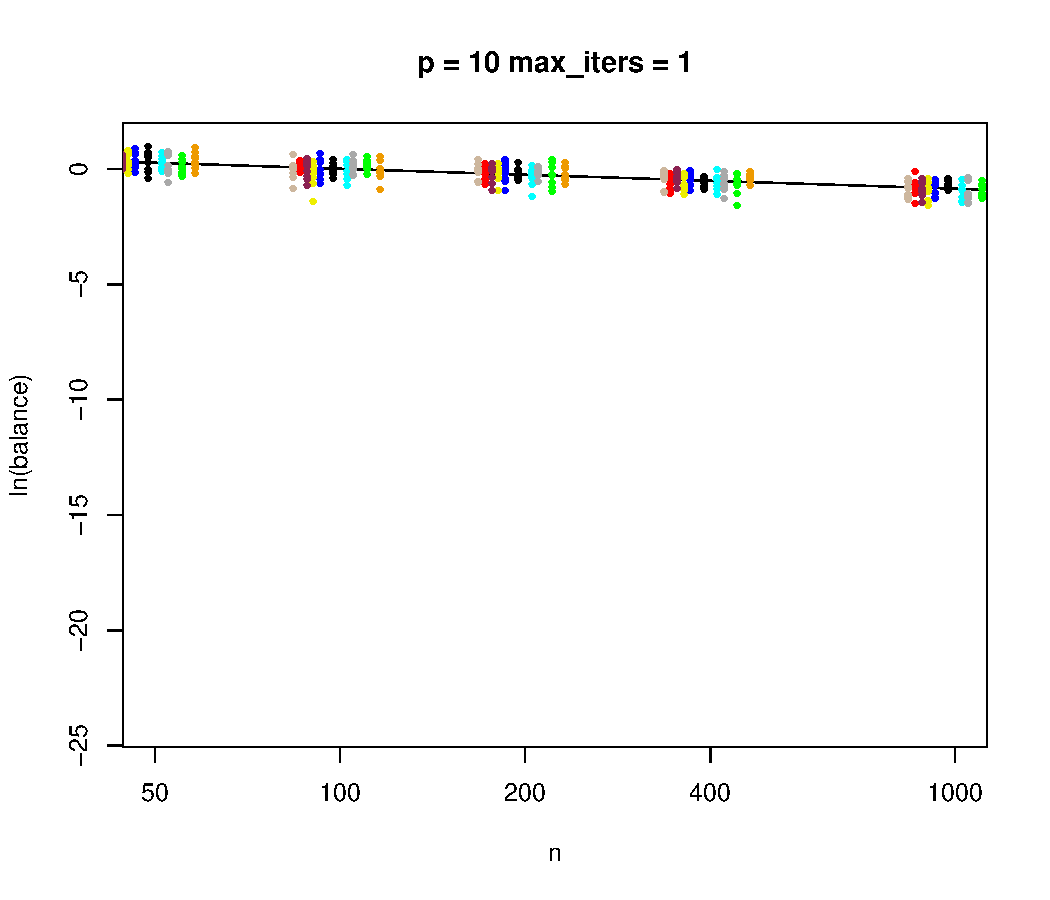
\includegraphics[width=\maxwidth]{figure/load_and_cleanup_data12} 
\begin{kframe}\begin{verbatim}
## p = 10 max iters = 1 
## 
## 
## examine log-log linear regression
##             Estimate Std. Error t value  Pr(>|t|)
## (Intercept)   1.7364    0.07628   22.76 3.777e-79
## lnx          -0.3757    0.01401  -26.81 1.131e-98
## ensure log-law relationship
## Analysis of Variance Table
## 
## Model 1: lny ~ poly(lnx, 1)
## Model 2: lny ~ poly(lnx, 4)
##   Res.Df  RSS Df Sum of Sq    F Pr(>F)
## 1    498 53.4                         
## 2    495 52.9  3     0.498 1.55    0.2
## ensure no dataset effect
## Analysis of Variance Table
## 
## Model 1: lny ~ lnx
## Model 2: lny ~ lnx + dataset
##   Res.Df  RSS Df Sum of Sq    F Pr(>F)
## 1    498 53.4                         
## 2    489 52.1  9      1.35 1.41   0.18
## Analysis of Variance Table
## 
## Model 1: lny ~ lnx
## Model 2: lny ~ lnx * dataset
##   Res.Df  RSS Df Sum of Sq    F Pr(>F)
## 1    498 53.4                         
## 2    480 51.5 18      1.95 1.01   0.45
\end{verbatim}
\end{kframe}
\end{knitrout}

\section{Multiple and Rate Results over all Runs}

% latex table generated in R 3.1.0 by xtable 1.7-4 package
% Sun Feb 15 16:48:02 2015
\begin{table}[ht]
\centering
\begin{tabular}{rrrrr}
  \hline
 & p & max\_iters & int & slope \\ 
  \hline
1 & 1.0000 &   Inf & 2.6479 & -3.1261 \\ 
  2 & 2.0000 &   Inf & 2.2401 & -1.9860 \\ 
  3 & 5.0000 &   Inf & 3.0409 & -1.4215 \\ 
  4 & 10.0000 &   Inf & 3.8644 & -1.2522 \\ 
  5 & 1.0000 & 2.0000 & -7.1018 & -0.6540 \\ 
  6 & 2.0000 & 2.0000 & -5.3310 & 0.0170 \\ 
  7 & 5.0000 & 2.0000 & -1.1958 & -0.1145 \\ 
  8 & 10.0000 & 2.0000 & 0.9213 & -0.2839 \\ 
  9 & 1.0000 & 1.0000 & -4.5420 & -0.5430 \\ 
  10 & 2.0000 & 1.0000 & -3.1601 & -0.0265 \\ 
  11 & 5.0000 & 1.0000 & 0.6113 & -0.3361 \\ 
  12 & 10.0000 & 1.0000 & 1.7364 & -0.3757 \\ 
   \hline
\end{tabular}
\end{table}

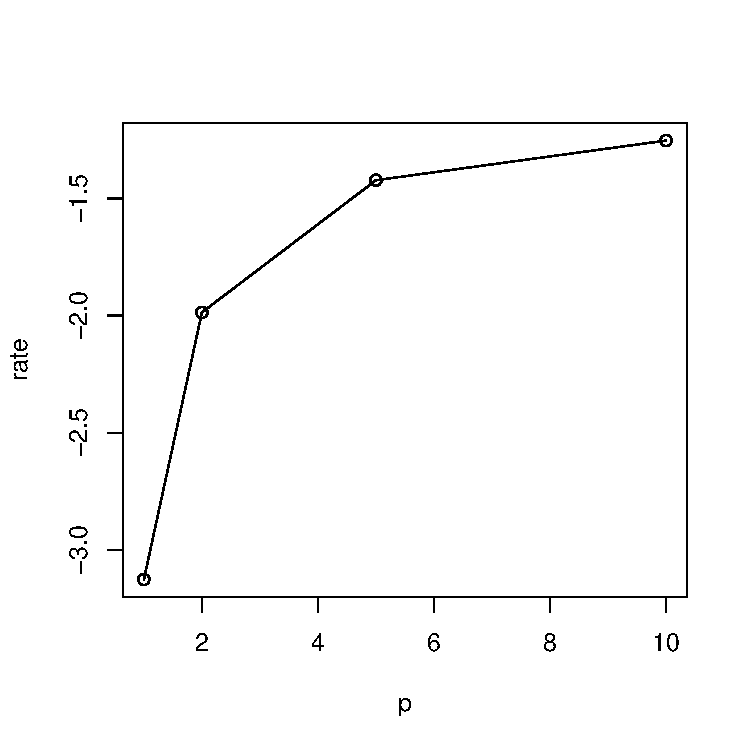
\includegraphics[width=\maxwidth]{figure/results_table} 





\end{document}

knit("sim_results.Rnw")
system("pdflatex sim_results.tex")
system("open sim_results.pdf")
